\providecommand{\main}{../../..}
\documentclass[\main/main.tex]{subfiles}
\begin{document}

\subsection{Esercizio 2}
Dato il problema di programmazione matematica

\begin{align*}
  \min f(x) & =x_2                       \\
  g_1(x)    & = x_1^2 + (x_2-1)^2 \leq 1 \\
  g_2(x)    & = x_1 - x_2 \leq -2
\end{align*}

\begin{enumerate}[a)]
  \item Si rappresenti il problema graficamente.
  \item Si determinino gli eventuali punti non regolari.
  \item Si determinino i punti candidati secondo le condizioni di KKT, e in particolare quello/i di minimo.
\end{enumerate}

\subsection{Soluzione esercizio 2}

\paragraph*{Riscrivo il problema}

\begin{align*}
  \min f(x) & =x_2                         \\
  g_1(x)    & = x_1^2 + x^2_2 -2x_2 \leq 0 \\
  g_2(x)    & = 2 + x_1 - x_2 \leq 0
\end{align*}

\paragraph*{Rappresentazione grafica del problema}

\begin{figure}
  \begin{subfigure}{0.45\textwidth}
    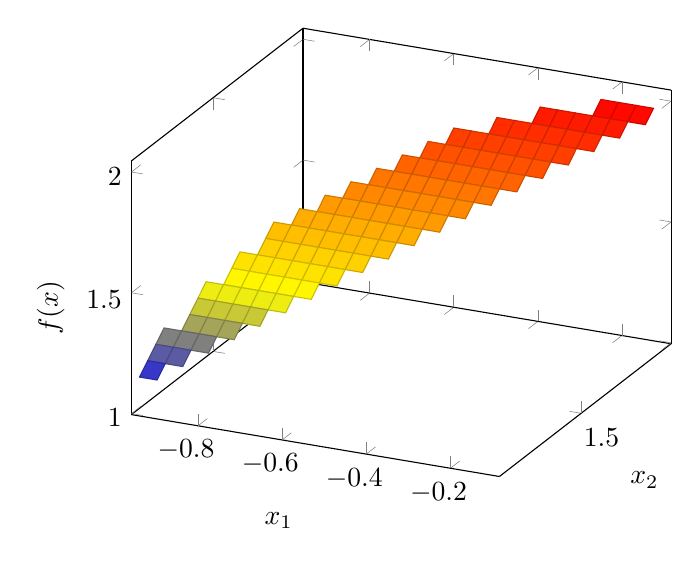
\begin{tikzpicture}
      \begin{axis}[
          xlabel=$x_1$,
          ylabel=$x_2$,
          zlabel=$f(x)$,
          domain=-1:0,
          y domain=1:2
        ]
        \addplot3[surf, unbounded coords=jump]
        {x^2 + y^2 -2*y <  0 && x - y < -2 ? y : NaN};
      \end{axis}
    \end{tikzpicture}
    \caption{La funzione $f(x)$}
    \label{func_1}
  \end{subfigure}
  ~
  \begin{subfigure}{0.45\textwidth}
    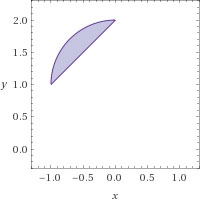
\includegraphics[width=0.8\textwidth]{14062016domain}
    \caption{Dominio della funzione $f(x)$}
  \end{subfigure}
\end{figure}

\paragraph*{Determino i punti non regolari}

\subparagraph*{Calcolo i gradienti dei vincoli}

\[
  \nabla g_1 = \begin{bmatrix}
    2x_1 \\
    2x_2 - 2
  \end{bmatrix}
  \qquad
  \nabla g_2 = \begin{bmatrix}
    1 \\
    -1
  \end{bmatrix}
\]

Il gradiente $\nabla g_1$ si annulla in $P = (0, 1)$ in cui il vincolo $g_1$ non è attivo ed è pertanto regolare. Il gradiente $\nabla g_2$ non si annulla mai.

\subparagraph*{Calcolo i punti di intersezione dei vincoli}

\[
  \begin{cases}
    x_1^2 + x^2_2 -2x_2 = 0 \\
    2 + x_1 - x_2 = 0
  \end{cases}
  \Rightarrow
  \begin{cases}
    (x_2 - 2)^2 + x^2_2 -2x_2 = 0 \\
    x_1 = x_2 - 2
  \end{cases}
  \Rightarrow
  \begin{cases}
    x^2_2 -4x_2 + 4 + x^2_2 -2x_2 = 0 \\
    x_1 = x_2 - 2
  \end{cases}
  \Rightarrow
  \begin{cases}
    x^2_2 -3x_2 + 2 = 0 \Rightarrow x_2 = \frac{3 \pm \sqrt{9 - 8}}{2} = \frac{3 \pm 1}{2} \\
    x_1 = x_2 - 2
  \end{cases}
\]

Dall'intersezione deriviamo i punti $A = (-1, 1)$ e $B = (0, 2)$. Sostituendo i punti nella matrice dei gradienti verifico che nè $A$ nè $B$ la rende singolare e sono pertanto regolari.

\paragraph*{Condizioni di KKT}

\subparagraph*{Costruisco la lagrangiana generalizzata}
\[
  l(x) = x_2 + \mu_1 (x_1^2 + x^2_2 -2x_2) + \mu_2 (2 + x_1 - x_2)
\]

\subparagraph*{Costruisco il sistema delle condizioni KKT}

\[
  \begin{cases}
    \nabla l(x) = \begin{bmatrix}
      2\mu_1x_1 + \mu_2 \\
      1 + \mu_1 (2x_2 - 2) - \mu_2
    \end{bmatrix}
    = \bm{0}                       \\
    \mu_1(x_1^2 + x^2_2 -2x_2) = 0 \\
    \mu_2(2 + x_1 - x_2) = 0       \\
    x_1^2 + x^2_2 -2x_2 \leq 0     \\
    2 + x_1 - x_2 \leq 0           \\
    \mu_1 \geq 0                   \\
    \mu_2 \geq 0
  \end{cases}
\]

Per risolvere il sistema procedo con un albero di bisezione sui vincoli, partendo dal più semplice, $\mu_2g_2$:

\subparagraph*{Caso $\mu_2 = 0 \land g_2 \leq 0$:}

\[
  \begin{cases}
    \nabla l(x) = \begin{bmatrix}
      2\mu_1x_1 \\
      1 + \mu_1 (2x_2 - 2)
    \end{bmatrix}
    = \bm{0} \Rightarrow x_1 = 0 \\
    \mu_1(x^2_2 -2x_2) = 0       \\
    x^2_2 -2x_2 \leq 0           \\
    2 - x_2 \leq 0               \\
    \mu_1 \geq 0
  \end{cases}
\]

Poichè $x_1 = 0$ è uno dei punti di intersezione dei vincoli, quindi $x_2 = 2$, altrimenti cadrebbe al di fuori del dominio.

\[
  \begin{cases}
    x_1 = 0                      \\
    x_2 = 2                      \\
    \error{\mu_1 = -\frac{1}{2}} \\
    \error{\mu_1 \geq 0}
  \end{cases}
\]

Il sistema risulta impossibile.

\subparagraph*{Caso $\mu_2 > 0 \land g_2 = 0$:}

\[
  \begin{cases}
    \nabla l(x) = \begin{bmatrix}
      2\mu_1(x_2 - 2) + \mu_2 \\
      1 + \mu_1 (2x_2 - 2) - \mu_2
    \end{bmatrix}
    = \bm{0}  \Rightarrow \mu_1 \neq 0 \\
    x_2^2  -3x_2 + 2 = 0               \\
    x_1 = x_2 - 2                      \\
    \mu_1 > 0                          \\
    \mu_2 > 0
  \end{cases}
  \Rightarrow
  \begin{cases}
    \begin{cases}
      \nabla l(x) = \begin{bmatrix}
        -2\mu_1 + \mu_2 \\
        1 - \mu_1 - \mu_2
      \end{bmatrix}
      = \bm{0}  \\
      \mu_2 > 0 \\
      x_2 = 1   \\
      x_1 = -1
    \end{cases}
    \Rightarrow
    \begin{cases}
      \mu_1 = \frac{\mu_2}{2}     \\
      \frac{\mu_2}{2} + \mu_2 = 1 \\
      \mu_2 > 0                   \\
      x_2 = 1                     \\
      x_1 = -1
    \end{cases}
    \Rightarrow
    \begin{cases}
      \mu_1 = \frac{1}{3} \\
      \mu_2 = \frac{2}{3} \\
      \mu_2 > 0           \\
      x_2 = 1             \\
      x_1 = -1
    \end{cases}
    \\
    \begin{cases}
      \error{\mu_2 = 0} \\
      \error{\mu_2 > 0} \\
      x_2 = 2           \\
      x_1 = 0
    \end{cases} \\
    \mu_1 > 0                  \\
  \end{cases}
\]

Le condizioni KKT eliminano il punto $B$ e confermano $A$ come punto candidato.

\subparagraph*{Sostituisco il valore numerico dei punti}
Il punto $A$ è l'ultimo candidato rimasto ed è quindi certamente l'ottimo locale. Questo è verificabile anche guardando il grafico della funzione in figura \ref{func_1}.

\[
  f(A) = f(-1, 1) = 1
\]


\end{document}